\documentclass{standalone}
\usepackage{tikz}
\usepackage{xcolor}
\usetikzlibrary{patterns, positioning}
\usetikzlibrary{shapes.misc}
\usepackage[outline]{contour}
\contourlength{1.5pt} 


\begin{document}
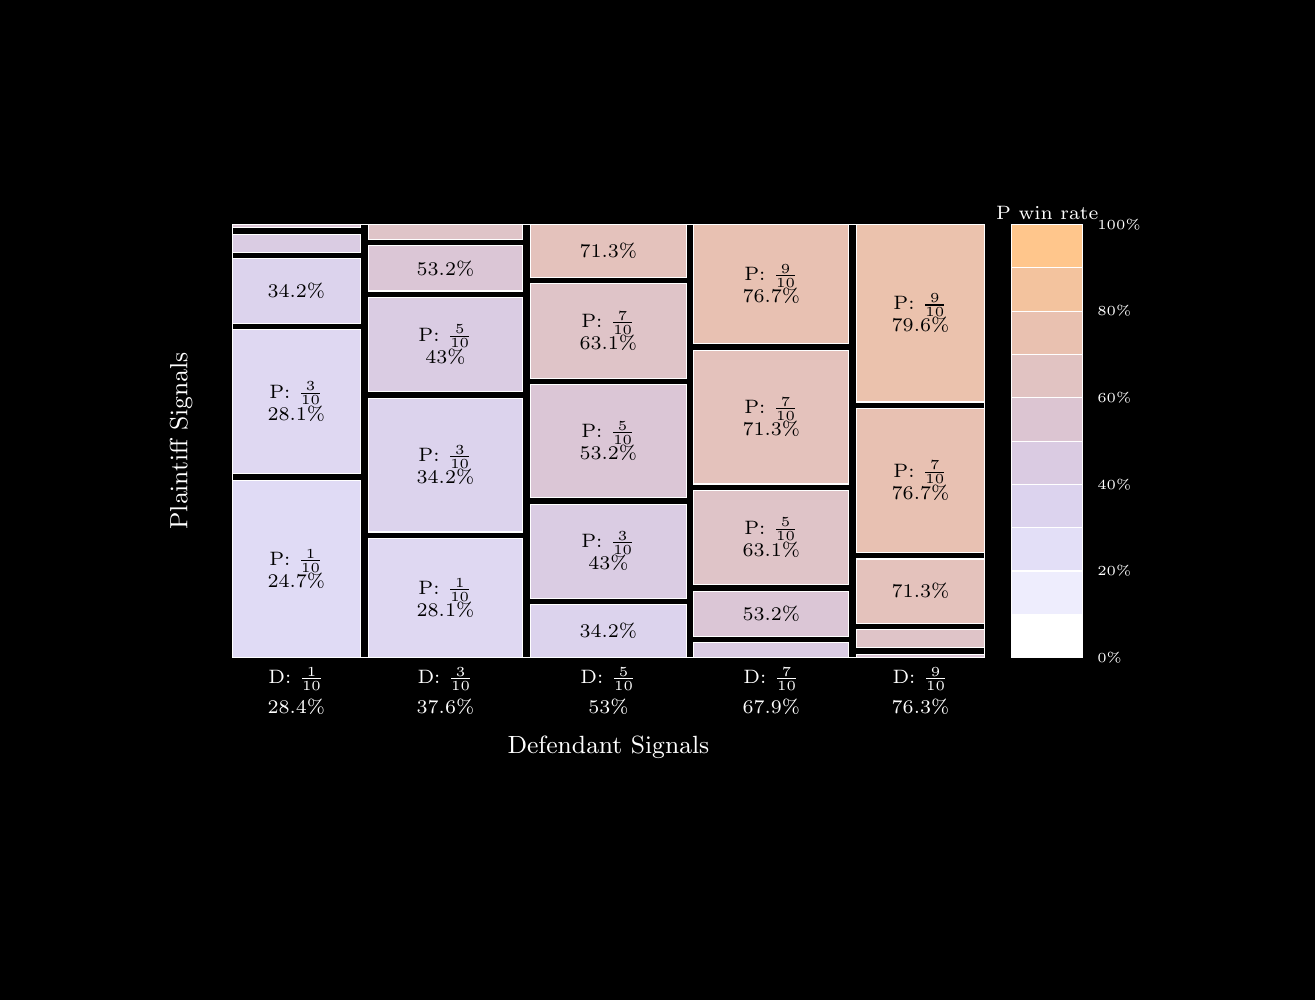
\begin{tikzpicture}
\newcommand{\DFractionOffset}{0.4}
\newcommand{\AxisLabelYAdjust}{-0.235}
\pagecolor{black}
\draw[fill=black, draw=none] (-2,-2) rectangle (14,10);
\draw[draw=white] (0.6,2) rectangle (10.15,7.5);
\draw[fill=blue!75!orange!25!white!64!white, draw=white] (0.6,2) rectangle (2.223,4.2536);
\draw (1.4114807963886014, 3.126779693792709) node[font=\scriptsize, text=black, align=center] {P: $\frac{1}{10}$\\ 24.7\%};
\draw[fill=blue!72!orange!28!white!63!white, draw=white] (0.6,4.3336) rectangle (2.223,6.1678);
\draw (1.4114807963886014, 5.250681257195448) node[font=\scriptsize, text=black, align=center] {P: $\frac{3}{10}$\\ 28.1\%};
\draw[fill=blue!66!orange!34!white!61!white, draw=white] (0.6,6.2478) rectangle (2.223,7.067);
\draw (1.4114807963886014, 6.657395456812517) node[font=\scriptsize, text=black, align=center] {34.2\%};
\draw[fill=blue!57!orange!43!white!59!white, draw=white] (0.6,7.147) rectangle (2.223,7.3765);
\draw[fill=blue!47!orange!53!white!57!white, draw=white] (0.6,7.4565) rectangle (2.223,7.5);
\draw (1.4114807963886014, 1.6) node[anchor=north, font=\scriptsize, text=white] {28.4\%};
\draw (1.4114807963886014, {1.6 + \DFractionOffset}) node[anchor=north, font=\scriptsize, text=white] {D: $\frac{1}{10}$};
\draw[fill=blue!72!orange!28!white!63!white, draw=white] (2.323,2) rectangle (4.2885,3.5145);
\draw (3.3057510410216735, 2.7572596413870145) node[font=\scriptsize, text=black, align=center] {P: $\frac{1}{10}$\\ 28.1\%};
\draw[fill=blue!66!orange!34!white!61!white, draw=white] (2.323,3.5945) rectangle (4.2885,5.2952);
\draw (3.3057510410216735, 4.444856889790416) node[font=\scriptsize, text=black, align=center] {P: $\frac{3}{10}$\\ 34.2\%};
\draw[fill=blue!57!orange!43!white!59!white, draw=white] (2.323,5.3752) rectangle (4.2885,6.5757);
\draw (3.3057510410216735, 5.975457703724756) node[font=\scriptsize, text=black, align=center] {P: $\frac{5}{10}$\\ 43\%};
\draw[fill=blue!47!orange!53!white!57!white, draw=white] (2.323,6.6557) rectangle (4.2885,7.2305);
\draw (3.3057510410216735, 6.943104220752757) node[font=\scriptsize, text=black, align=center] {53.2\%};
\draw[fill=blue!37!orange!63!white!54!white, draw=white] (2.323,7.3105) rectangle (4.2885,7.5);
\draw (3.3057510410216735, 1.6) node[anchor=north, font=\scriptsize, text=white] {37.6\%};
\draw (3.3057510410216735, {1.6 + \DFractionOffset}) node[anchor=north, font=\scriptsize, text=white] {D: $\frac{3}{10}$};
\draw[fill=blue!66!orange!34!white!61!white, draw=white] (4.3885,2) rectangle (6.3615,2.6739);
\draw (5.375, 2.33693862396999) node[font=\scriptsize, text=black, align=center] {34.2\%};
\draw[fill=blue!57!orange!43!white!59!white, draw=white] (4.3885,2.7539) rectangle (6.3615,3.9499);
\draw (5.375, 3.351907212179956) node[font=\scriptsize, text=black, align=center] {P: $\frac{3}{10}$\\ 43\%};
\draw[fill=blue!47!orange!53!white!57!white, draw=white] (4.3885,4.0299) rectangle (6.3615,5.4701);
\draw (5.375, 4.75) node[font=\scriptsize, text=black, align=center] {P: $\frac{5}{10}$\\ 53.2\%};
\draw[fill=blue!37!orange!63!white!54!white, draw=white] (4.3885,5.5501) rectangle (6.3615,6.7461);
\draw (5.375, 6.148092787820044) node[font=\scriptsize, text=black, align=center] {P: $\frac{7}{10}$\\ 63.1\%};
\draw[fill=blue!29!orange!71!white!52!white, draw=white] (4.3885,6.8261) rectangle (6.3615,7.5);
\draw (5.375, 7.16306137603001) node[font=\scriptsize, text=black, align=center] {71.3\%};
\draw (5.375, 1.6) node[anchor=north, font=\scriptsize, text=white] {53\%};
\draw (5.375, {1.6 + \DFractionOffset}) node[anchor=north, font=\scriptsize, text=white] {D: $\frac{5}{10}$};
\draw[fill=blue!57!orange!43!white!59!white, draw=white] (6.4615,2) rectangle (8.427,2.1895);
\draw[fill=blue!47!orange!53!white!57!white, draw=white] (6.4615,2.2695) rectangle (8.427,2.8443);
\draw (7.444248958978325, 2.556895779247243) node[font=\scriptsize, text=black, align=center] {53.2\%};
\draw[fill=blue!37!orange!63!white!54!white, draw=white] (6.4615,2.9243) rectangle (8.427,4.1248);
\draw (7.444248958978325, 3.5245422962752455) node[font=\scriptsize, text=black, align=center] {P: $\frac{5}{10}$\\ 63.1\%};
\draw[fill=blue!29!orange!71!white!52!white, draw=white] (6.4615,4.2048) rectangle (8.427,5.9055);
\draw (7.444248958978325, 5.055143110209584) node[font=\scriptsize, text=black, align=center] {P: $\frac{7}{10}$\\ 71.3\%};
\draw[fill=blue!23!orange!77!white!51!white, draw=white] (6.4615,5.9855) rectangle (8.427,7.5);
\draw (7.444248958978325, 6.742740358612985) node[font=\scriptsize, text=black, align=center] {P: $\frac{9}{10}$\\ 76.7\%};
\draw (7.444248958978325, 1.6) node[anchor=north, font=\scriptsize, text=white] {67.9\%};
\draw (7.444248958978325, {1.6 + \DFractionOffset}) node[anchor=north, font=\scriptsize, text=white] {D: $\frac{7}{10}$};
\draw[fill=blue!47!orange!53!white!57!white, draw=white] (8.527,2) rectangle (10.15,2.0435);
\draw[fill=blue!37!orange!63!white!54!white, draw=white] (8.527,2.1235) rectangle (10.15,2.353);
\draw[fill=blue!29!orange!71!white!52!white, draw=white] (8.527,2.433) rectangle (10.15,3.2522);
\draw (9.338519203611398, 2.842604543187483) node[font=\scriptsize, text=black, align=center] {71.3\%};
\draw[fill=blue!23!orange!77!white!51!white, draw=white] (8.527,3.3322) rectangle (10.15,5.1664);
\draw (9.338519203611398, 4.249318742804552) node[font=\scriptsize, text=black, align=center] {P: $\frac{7}{10}$\\ 76.7\%};
\draw[fill=blue!20!orange!80!white!50!white, draw=white] (8.527,5.2464) rectangle (10.15,7.5);
\draw (9.338519203611398, 6.3732203062072905) node[font=\scriptsize, text=black, align=center] {P: $\frac{9}{10}$\\ 79.6\%};
\draw (9.338519203611398, 1.6) node[anchor=north, font=\scriptsize, text=white] {76.3\%};
\draw (9.338519203611398, {1.6 + \DFractionOffset}) node[anchor=north, font=\scriptsize, text=white] {D: $\frac{9}{10}$};
\node[font=\small, text=white] at (5.375, {1.1 + \AxisLabelYAdjust}) {Defendant Signals};
\node[font=\small, text=white, rotate=90] at (-0.050000000000000044, 4.75) {Plaintiff Signals};
\draw[draw=white] (10.5,2) rectangle (11.4,7.5);
\draw (10.95, 7.65) node[font=\scriptsize, text=white] {P win rate};
\draw[fill=blue!100!orange!0!white!70!white, draw=white] (10.5,2) rectangle (11.4,2.55);
\draw[fill=blue!89!orange!11!white!67!white, draw=white] (10.5,2.55) rectangle (11.4,3.1);
\draw[fill=blue!78!orange!22!white!64!white, draw=white] (10.5,3.1) rectangle (11.4,3.65);
\draw[fill=blue!67!orange!33!white!62!white, draw=white] (10.5,3.65) rectangle (11.4,4.2);
\draw[fill=blue!56!orange!44!white!59!white, draw=white] (10.5,4.2) rectangle (11.4,4.75);
\draw[fill=blue!44!orange!56!white!56!white, draw=white] (10.5,4.75) rectangle (11.4,5.3);
\draw[fill=blue!33!orange!67!white!53!white, draw=white] (10.5,5.3) rectangle (11.4,5.85);
\draw[fill=blue!22!orange!78!white!51!white, draw=white] (10.5,5.85) rectangle (11.4,6.4);
\draw[fill=blue!11!orange!89!white!48!white, draw=white] (10.5,6.4) rectangle (11.4,6.95);
\draw[fill=blue!0!orange!100!white!45!white, draw=white] (10.5,6.95) rectangle (11.4,7.5);
\draw (11.46, 2) node[anchor=west, font=\tiny, text=white] {0\%};
\draw (11.46, 3.1) node[anchor=west, font=\tiny, text=white] {20\%};
\draw (11.46, 4.2) node[anchor=west, font=\tiny, text=white] {40\%};
\draw (11.46, 5.3) node[anchor=west, font=\tiny, text=white] {60\%};
\draw (11.46, 6.4) node[anchor=west, font=\tiny, text=white] {80\%};
\draw (11.46, 7.5) node[anchor=west, font=\tiny, text=white] {100\%};


\end{tikzpicture}
\end{document}